\documentclass[1,DS,p,e,prof]{phBook}
%\documentclass[../coursseconde]{subfiles}
%Options : 2, 1, T, SNT (classes), p, b,prof, exos, cours, DS, noir, a4, a5, twocolumn, landscape
\def\datedevoir{6/01/26} % date du DS à indiquer

\graphicspath{{figures/}}

\begin{document}
\setcounter{chapter}{3} %Numéro du chapitre précédent
\chapter{\prof{CORRECTION}\eleve{NOM : \hfill Devoir
}} %Titre du chapitre
%%%%%%%%%%%%%%%%%%%%%%%%

\begin{exercice}
    \begin{enonce}
        Pour chacune des fonctions suivantes :
        \begin{itemize}
            \item Calculer la dérivée \(f'(x)\).
            % \item Étudier le signe de \(f'(x)\).
            \item Déterminer les sens de variations de la fonction \(f\).
        \end{itemize}
        \begin{enumerate}
            \item \(f(x)=x^2-4x+3\).
            \item \(f(x)=-2x^2+4x+5\).
            \item \(f(x)=-x^3+3x^2-3x+2\).
            % \item \(f(x)=x^3-6x^2+9x+1\).
            \item \(f(x)=-2x^3+3x^2+12x-5\).
            \item \(f(x)=\dfrac{2x+1}{x-2}\) définie sur \(\mathbb{R}\setminus\{2\}\).
            \item \(f(x)=3x+\dfrac{48}{x}\), définie sur \(\mathbb{R}\setminus\{0\}\).
        \end{enumerate}
    \end{enonce}
    \begin{correction} % assistée par IA
        \begin{enumerate}
            \item $f(x)=x^2-4x+3$
            
            \textbf{Dérivée :} $f'(x)=2x-4$
            % Calcul vérifié
            
            \textbf{Signe de $f'(x)$ :} $f'(x)=0 \Leftrightarrow 2x-4=0 \Leftrightarrow x=2$
            
            $f'(x)<0$ si $x<2$ et $f'(x)>0$ si $x>2$
            
            \textbf{Tableau de variations :}
            \begin{center}
              \begin{tikzpicture}[scale=0.7]
              \tkzTabInit[lgt=2,espcl=2]{$x$/1, $f'(x)$/1, $f(x)$/2}{$-\infty$, $2$, $+\infty$}
              \tkzTabLine{, -, z, +, }
              \tkzTabVar{+/, -/$-1$, +/}
              \end{tikzpicture}
            \end{center}
            % Calcul vérifié : f(2) = 4 - 8 + 3 = -1
            
            $f$ est décroissante sur $]-\infty;2]$ et croissante sur $[2;+\infty[$.
            
            \item $f(x)=-2x^2+4x+5$
            
            \textbf{Dérivée :} $f'(x)=-4x+4$
            % Calcul vérifié
            
            \textbf{Signe de $f'(x)$ :} $f'(x)=0 \Leftrightarrow -4x+4=0 \Leftrightarrow x=1$
            
            $f'(x)>0$ si $x<1$ et $f'(x)<0$ si $x>1$
            
            \textbf{Tableau de variations :}
            \begin{center}
              \begin{tikzpicture}[scale=0.7]
              \tkzTabInit[lgt=2,espcl=2]{$x$/1, $f'(x)$/1, $f(x)$/2}{$-\infty$, $1$, $+\infty$}
              \tkzTabLine{, +, z, -, }
              \tkzTabVar{-/, +/$7$, -/}
              \end{tikzpicture}
            \end{center}
            % Calcul vérifié : f(1) = -2 + 4 + 5 = 7
            
            $f$ est croissante sur $]-\infty;1]$ et décroissante sur $[1;+\infty[$.
            
            \item $f(x)=-x^3+3x^2-3x+2$
            
            \textbf{Dérivée :} $f'(x)=-3x^2+6x-3=-3(x^2-2x+1)=-3(x-1)^2$
            % Calcul vérifié
            
            \textbf{Signe de $f'(x)$ :} $f'(x)=-3(x-1)^2 \leq 0$ pour tout $x \in \mathbb{R}$
            
            $f'(x)=0$ seulement pour $x=1$
            
            \textbf{Tableau de variations :}
            \begin{center}
              \begin{tikzpicture}[scale=0.7]
              \tkzTabInit[lgt=2,espcl=2]{$x$/1, $f'(x)$/1, $f(x)$/2}{$-\infty$, $1$, $+\infty$}
              \tkzTabLine{, -, z, -, }
              \tkzTabVar{+/, -/$1$, -/}
              \end{tikzpicture}
            \end{center}
            % Calcul vérifié : f(1) = -1 + 3 - 3 + 2 = 1
            
            $f$ est décroissante sur $\mathbb{R}$.
            
            \item $f(x)=-2x^3+3x^2+12x-5$
            
            \textbf{Dérivée :} $f'(x)=-6x^2+6x+12=-6(x^2-x-2)$
            % Calcul vérifié
            
            \textbf{Signe de $f'(x)$ :} Étudions le signe de $x^2-x-2$.
            
            $\Delta = (-1)^2-4(1)(-2)=1+8=9>0$
            % Calcul vérifié
            
            Racines : $x_1=\dfrac{1-3}{2}=-1$ et $x_2=\dfrac{1+3}{2}=2$
            % Calcul vérifié
            
            Donc $x^2-x-2=(x+1)(x-2)$ et $f'(x)=-6(x+1)(x-2)$
            
            $f'(x)>0$ si $-1<x<2$ et $f'(x)<0$ si $x<-1$ ou $x>2$
            
            \textbf{Tableau de variations :}
            \begin{center}
              \begin{tikzpicture}[scale=0.7]
              \tkzTabInit[lgt=2,espcl=2]{$x$/1, $f'(x)$/1, $f(x)$/2}{$-\infty$, $-1$, $2$, $+\infty$}
              \tkzTabLine{, -, z, +, z, -, }
              \tkzTabVar{+/, -/$-12$, +/$15$, -/}
              \end{tikzpicture}
            \end{center}
            % Calcul vérifié : f(-1) = 2 + 3 - 12 - 5 = -12
            % Calcul vérifié : f(2) = -16 + 12 + 24 - 5 = 15
            
            $f$ est décroissante sur $]-\infty;-1]$ et sur $[2;+\infty[$, croissante sur $[-1;2]$.
            
            \item $f(x)=\dfrac{2x+1}{x-2}$ sur $\mathbb{R}\setminus\{2\}$
            
            \textbf{Dérivée :} $f'(x)=\dfrac{2(x-2)-(2x+1)(1)}{(x-2)^2}=\dfrac{2x-4-2x-1}{(x-2)^2}=\dfrac{-5}{(x-2)^2}$
            % Calcul vérifié
            
            \textbf{Signe de $f'(x)$ :} $f'(x)=\dfrac{-5}{(x-2)^2}<0$ pour tout $x \neq 2$
            
            \textbf{Tableau de variations :}
            \begin{center}
              \begin{tikzpicture}[scale=0.7]
              \tkzTabInit[lgt=2,espcl=2]{$x$/1, $f'(x)$/1, $f(x)$/2}{$-\infty$, $2$, $+\infty$}
              \tkzTabLine{, -, d, -, }
              \tkzTabVar{+/, -D+//, -/}
              \end{tikzpicture}
            \end{center}
            
            $f$ est décroissante sur $]-\infty;2[$ et sur $]2;+\infty[$.
            
            \item $f(x)=3x+\dfrac{48}{x}$ sur $\mathbb{R}\setminus\{0\}$
            
            \textbf{Dérivée :} $f'(x)=3-\dfrac{48}{x^2}=\dfrac{3x^2-48}{x^2}$
            % Calcul vérifié
            
            \textbf{Signe de $f'(x)$ :} $f'(x)=0 \Leftrightarrow 3x^2-48=0 \Leftrightarrow x^2=16 \Leftrightarrow x=\pm 4$
            % Calcul vérifié
            
            $f'(x)>0$ si $x<-4$ ou $x>4$, et $f'(x)<0$ si $-4<x<0$ ou $0<x<4$
            
            \textbf{Tableau de variations :}
            \begin{center}
              \begin{tikzpicture}[scale=0.7]
              \tkzTabInit[lgt=2,espcl=2]{$x$/1, $f'(x)$/1, $f(x)$/2}{$-\infty$, $-4$, $0$, $4$, $+\infty$}
              \tkzTabLine{, +, z, -, d, -, z, +, }
              \tkzTabVar{-/, +/$-24$, -D+//, -/$24$, +/}
              \end{tikzpicture}
            \end{center}
            % Calcul vérifié : f(-4) = -12 - 12 = -24
            % Calcul vérifié : f(4) = 12 + 12 = 24
            
            $f$ est croissante sur $]-\infty;-4]$ et sur $[4;+\infty[$, décroissante sur $[-4;0[$ et sur $]0;4]$.
        \end{enumerate}
    \end{correction}
\end{exercice}
%%%%%%%%%%%%%%%%%
% Fin exercice %%
%%%%%%%%%%%%%%%%%



\begin{exercice}
    \begin{enonce}
        Donner les variations de $f(x)=\frac{2x-1}{x+3}$ sur son domaine de définition.
    \end{enonce}
    \begin{correction} % assistée par IA
        \textbf{Domaine de définition :} $\mathcal{D}_f = \mathbb{R}\setminus\{-3\}$
        
        \textbf{Dérivée :} $f'(x)=\dfrac{2(x+3)-(2x-1)(1)}{(x+3)^2}=\dfrac{2x+6-2x+1}{(x+3)^2}=\dfrac{7}{(x+3)^2}$
        % Calcul vérifié
        
        \textbf{Signe de $f'(x)$ :} $f'(x)=\dfrac{7}{(x+3)^2}>0$ pour tout $x \neq -3$
        
        \textbf{Tableau de variations :}
        \begin{center}
          \begin{tikzpicture}[scale=0.7]
          \tkzTabInit[lgt=2,espcl=2]{$x$/1, $f'(x)$/1, $f(x)$/2}{$-\infty$, $-3$, $+\infty$}
          \tkzTabLine{, +, d, +, }
          \tkzTabVar{-/, +D-//, +/}
          \end{tikzpicture}
        \end{center}
        
        $f$ est strictement croissante sur $]-\infty;-3[$ et sur $]-3;+\infty[$.
    \end{correction}
\end{exercice}
%%%%%%%%%%%%%%%%%%%%%
%%% Fin exercice %%%%
%%%%%%%%%%%%%%%%%%%%%

\end{document}